
\section{Netzwerke}
Netzwerke setzen sich im allgmeinen aus $N$ Knoten (Nodes) zusammen, die über gewichtete Verbindungen (Edges) miteinander verbunden sind. Besteht zwischen zwei Knoten eine Verbindung in beide Richtungen, so spricht man von einem ungerichteten Netzwerk. Wenn alle Knoten untereinander verbunden sind, so handelt es sich um ein vollständiges Netzwerk (siehe Abbildung \ref{fig:GraphBsp}). Die Verbindungen der Knoten lassen sich durch eine MxM Verbindungsmatrix $\boldsymbol{A}$ darstellen, in der ein Eintrag von $1$ an Position $i,j$ eine Verbindung zwischen dem Knoten $i$ und dem Knoten $j$, eine $0$ keine Verbindung zwischen diesen Knoten bedeutet.

\begin{figure}[t]
	 \centering
	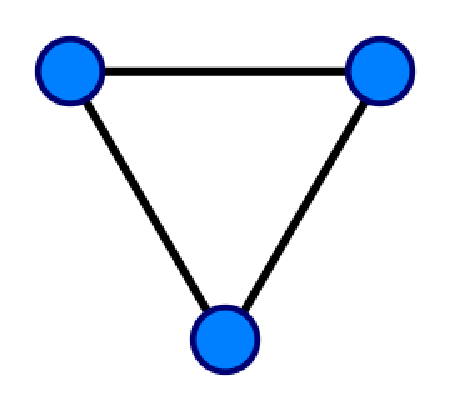
\includegraphics[width=0.25\textwidth]{abb/misc/GraphBsp.eps}
	\caption[Ungerichteres Netzwerk]{Beispiel eines ungerichteten Netzwerks aus vier Knoten, bei dem jeder Knoten mit jedem anderen verbunden ist.}
	\label{fig:GraphBsp}
\end{figure}


\subsection*{Dynamik auf Netzwerken}
Um Prozesse auf Netzwerken zu beschreiben kann man jedem Knoten eine $n$-dimensionale dynamische Variable $x_i$ zuordnen. Die Dynamik wird dann für jeden Knoten über eine Differentialgleichung beschrieben, die die Kopplung an die anderen Knoten enthält. Die allgemeine Form dieser Differentialgleichung ist für ein System ohne Rückkopplung in Gleichung (\ref*{eq:dyneqcommon}) gezeigt.

%was ist das mit der rückkopplung? die ist doch da drin?
XXXX

\begin{align}\label{eq:dyneqcommon}
\overset{\cdot}{\boldsymbol{x}}_i(t)&=\boldsymbol{f}(\boldsymbol{x}_i(t))+\sigma\sum_j A_{ij}\boldsymbol{h}\left(\boldsymbol{x}_j(t)\right)
\\\notag & i=1,...,N
\\\notag & \sigma \text{ allgemeine Kopplungsstärke}
\\\notag & A_{ij}\text{ Element der Kopplungsmatrix}
\\\notag & \boldsymbol{f},\boldsymbol{h}:\mathbb{R}^n\rightarrow\mathbb{R}^n
\end{align}
Die Verbindungsmatrix $\boldsymbol{A}$ wird hierbei zu einer Kopplungsmatrix, die die Kopplung der Differentialgleichungen der Knoten untereinander beschreibt. Im folgenden werden nur solche Systeme betrachtete, bei denen $\boldsymbol{A}$ symmetrisch ist, das Netzwerk also ungerichtet. Die Abbildung $\boldsymbol{h}$ beschreibt auf welche Art und Weise die Komponenten der Variablen $\boldsymbol{x}_i$ aneinander koppeln. Das Differentialgleichungssystem in (\ref*{eq:dyneqcommon}) lässt sich auch über das Kronecker-Produkt in einer einzigen Gleichung darstellen \citep{pecora1998},
\begin{align}
\overset{\cdot}{\boldsymbol{X}}(t)=\boldsymbol{F}(\boldsymbol{X}(t))+\sigma\boldsymbol{A}\otimes\boldsymbol{H}(\boldsymbol{X}(t))
\end{align}
mit den Definitionen:
\begin{align*}
\boldsymbol{X}=\left(\boldsymbol{x}_1,...,\boldsymbol{x}_N\right)^{\text{T}},
\boldsymbol{F}=\left(\boldsymbol{f}(\boldsymbol{x}_1),...,\boldsymbol{f}(\boldsymbol{x}_N)\right)^{\text{T}},
\boldsymbol{H}=\left(\boldsymbol{h}(\boldsymbol{x}_1),...,\boldsymbol{h}(\boldsymbol{x}_N)\right)^{\text{T}}
\end{align*}

